\insertdesignoverview{Duck Spinner}
{Make a small, low profile mechanism that is fast enough to spin all of the ducks around the carousel during endgame. Additionally, the duck spinner should be strong because of its collisions with the carousel.} % Goals of the mechanism
{Hang.PNG}% CAD Image
{fullbullseyehang.PNG}% Build Image
{Medical Grade Polycarbonate, Plastic Paint Roller Tube, Andymark Sushi Roller}% Materials ex. 0.25" MDF, Aluminum, etc
{3D Printing}% Manufacturing Processes ex. Laser Cut, 3D print, etc.

%\interesting{Our innovative glyph delivery mechanism, analyzed in depth}{Innovate:55}

\subsection*{How it Works}
Attached at the front of the robot, the Duck spinner was created to easily drive up to the carousel and spin all of the ducks off as quickly as possible. The main structure of the duck spinner is made out of the plastic inside of a paint roller. The paint roller was chosen for its shape and strength. Inside the paint roller is an Andymark Neverrest motor without a gearbox, allowing it to rotate at a speed of about six thousand RPM. because this is so fast that it throws the ducks off the carousel, we reduce the speed to the perfect angular velocity to spin the carousel without launching the ducks off. The motor is connected to a tiny wheel, called a sushi roller, at the top. We chose the sushi roller over a compliant wheel to keep the profile low. An added benefit of the sushi roller is that it is less squishy than a compliant wheel which prevents the robot from bouncing off the carousel if it hits it at a high speed. To hold everything together, there are 3D printed parts at the top and bottom of the duck spinner.
% Design_Spinner_Image1

%  \begin{figure}[h!]
%  \centering
%    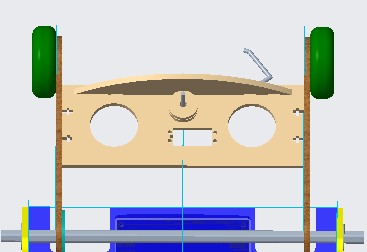
\includegraphics[width=0.8\textwidth, angle=0]{Design_Overview/Hang_1.PNG}
%   \caption{Hang Top Pic}
%   \label{fig:hang_top}
%  \end{figure}

% \subsection*{Modelling \& Simulation}
% Modelling the hang mechanism involved minimal design challenges. The only thing we originally struggled with was how the arms would line up with the lander. In order to model this, we used body and motion skeletons to see the distance to the latch as well as how far in it would reach. However, issues were primarily resolved through design iteration, as you'll see below. 

% \subsection*{Iteration}
% Initially,we angled the hang plate that held the hook, believing that that would allow for the hook to be well within the latch. However, after testing, we determined that a straight hang plate worked much better. We also made several iterations of a winch box that would rest at the back of the chassis, yet after struggling with space issues we realized that we could simply mount the motor directly on the underbelly of the chassis with a hole to guide the winch string.

% \begin{figure}[htp]
% \centering
% 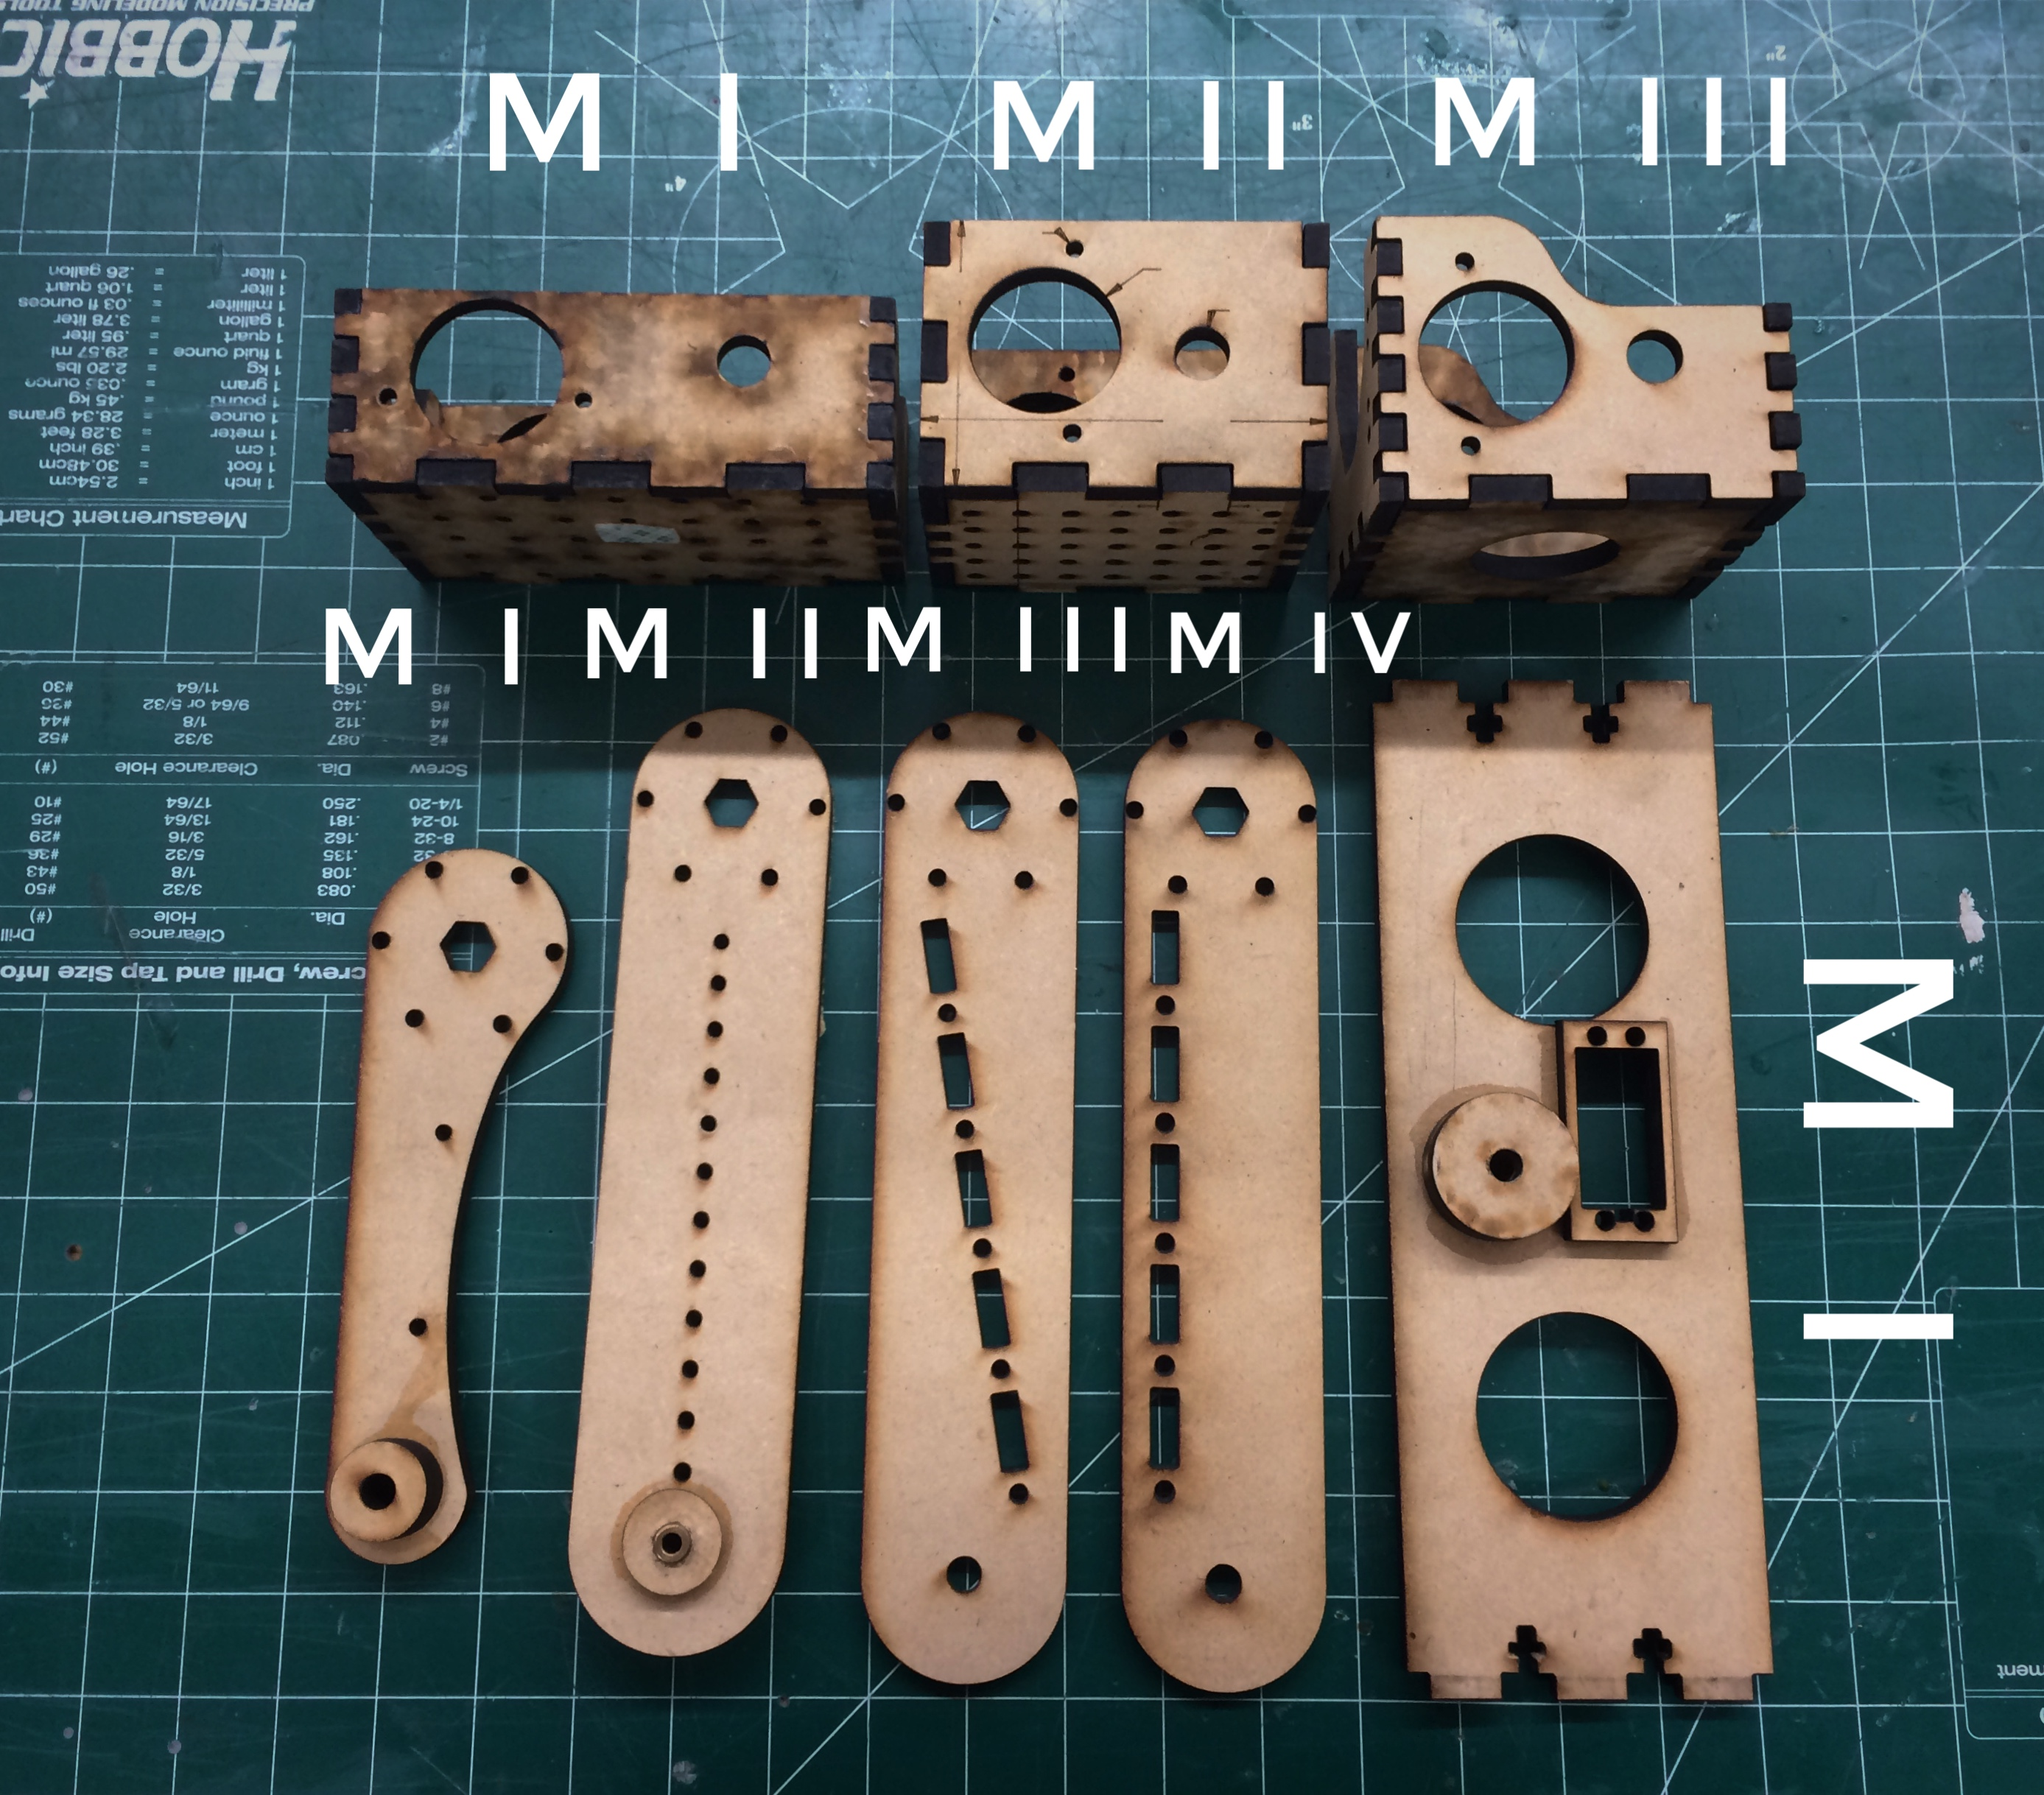
\includegraphics[width=.8\linewidth]{Design_Overview/Hang_Iteration.jpg}
% \caption{Design Iteration of the Hang, Mark I to Mark IV}
% \label{fig:hang_iteration}
% \end{figure}

% \begin{figure}[htp]
% \centering
% \begin{minipage}{.32\textwidth}
%   \centering
%   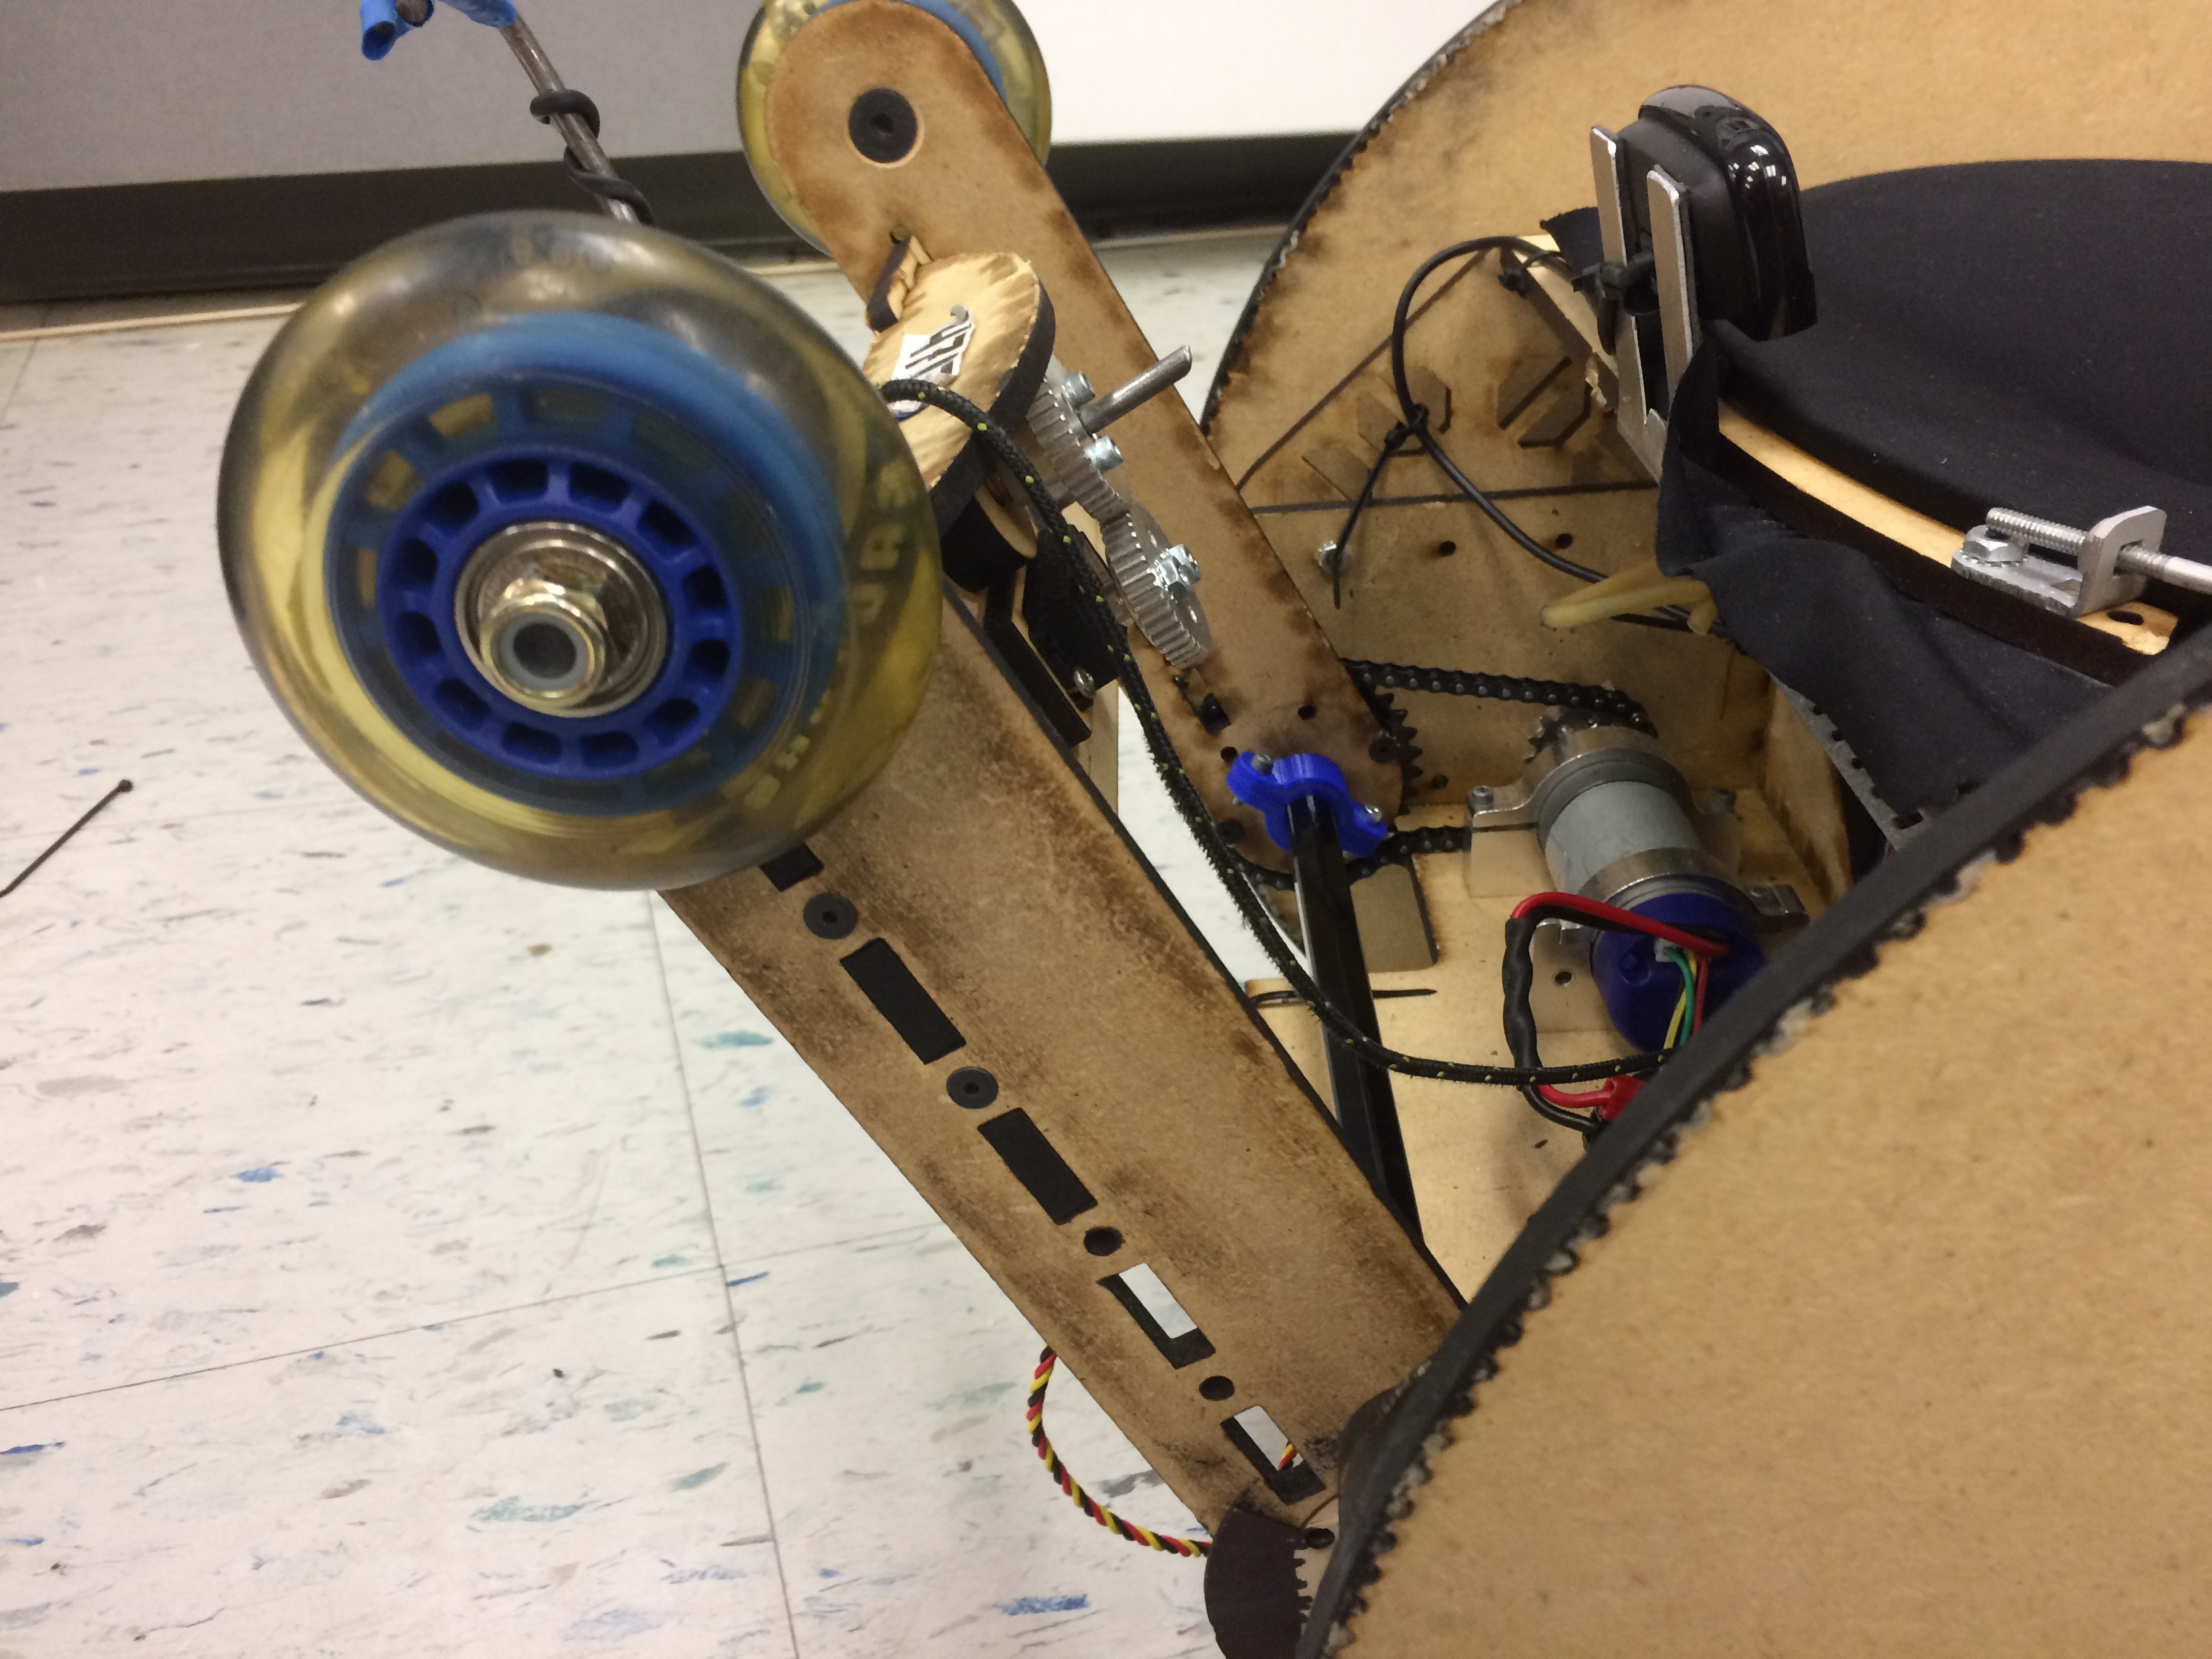
\includegraphics[width= .9\linewidth]{Design_Overview/Hang_Left.JPG}
% \end{minipage}%
% \hfill
% \begin{minipage}{.32\textwidth}
%   \centering
%   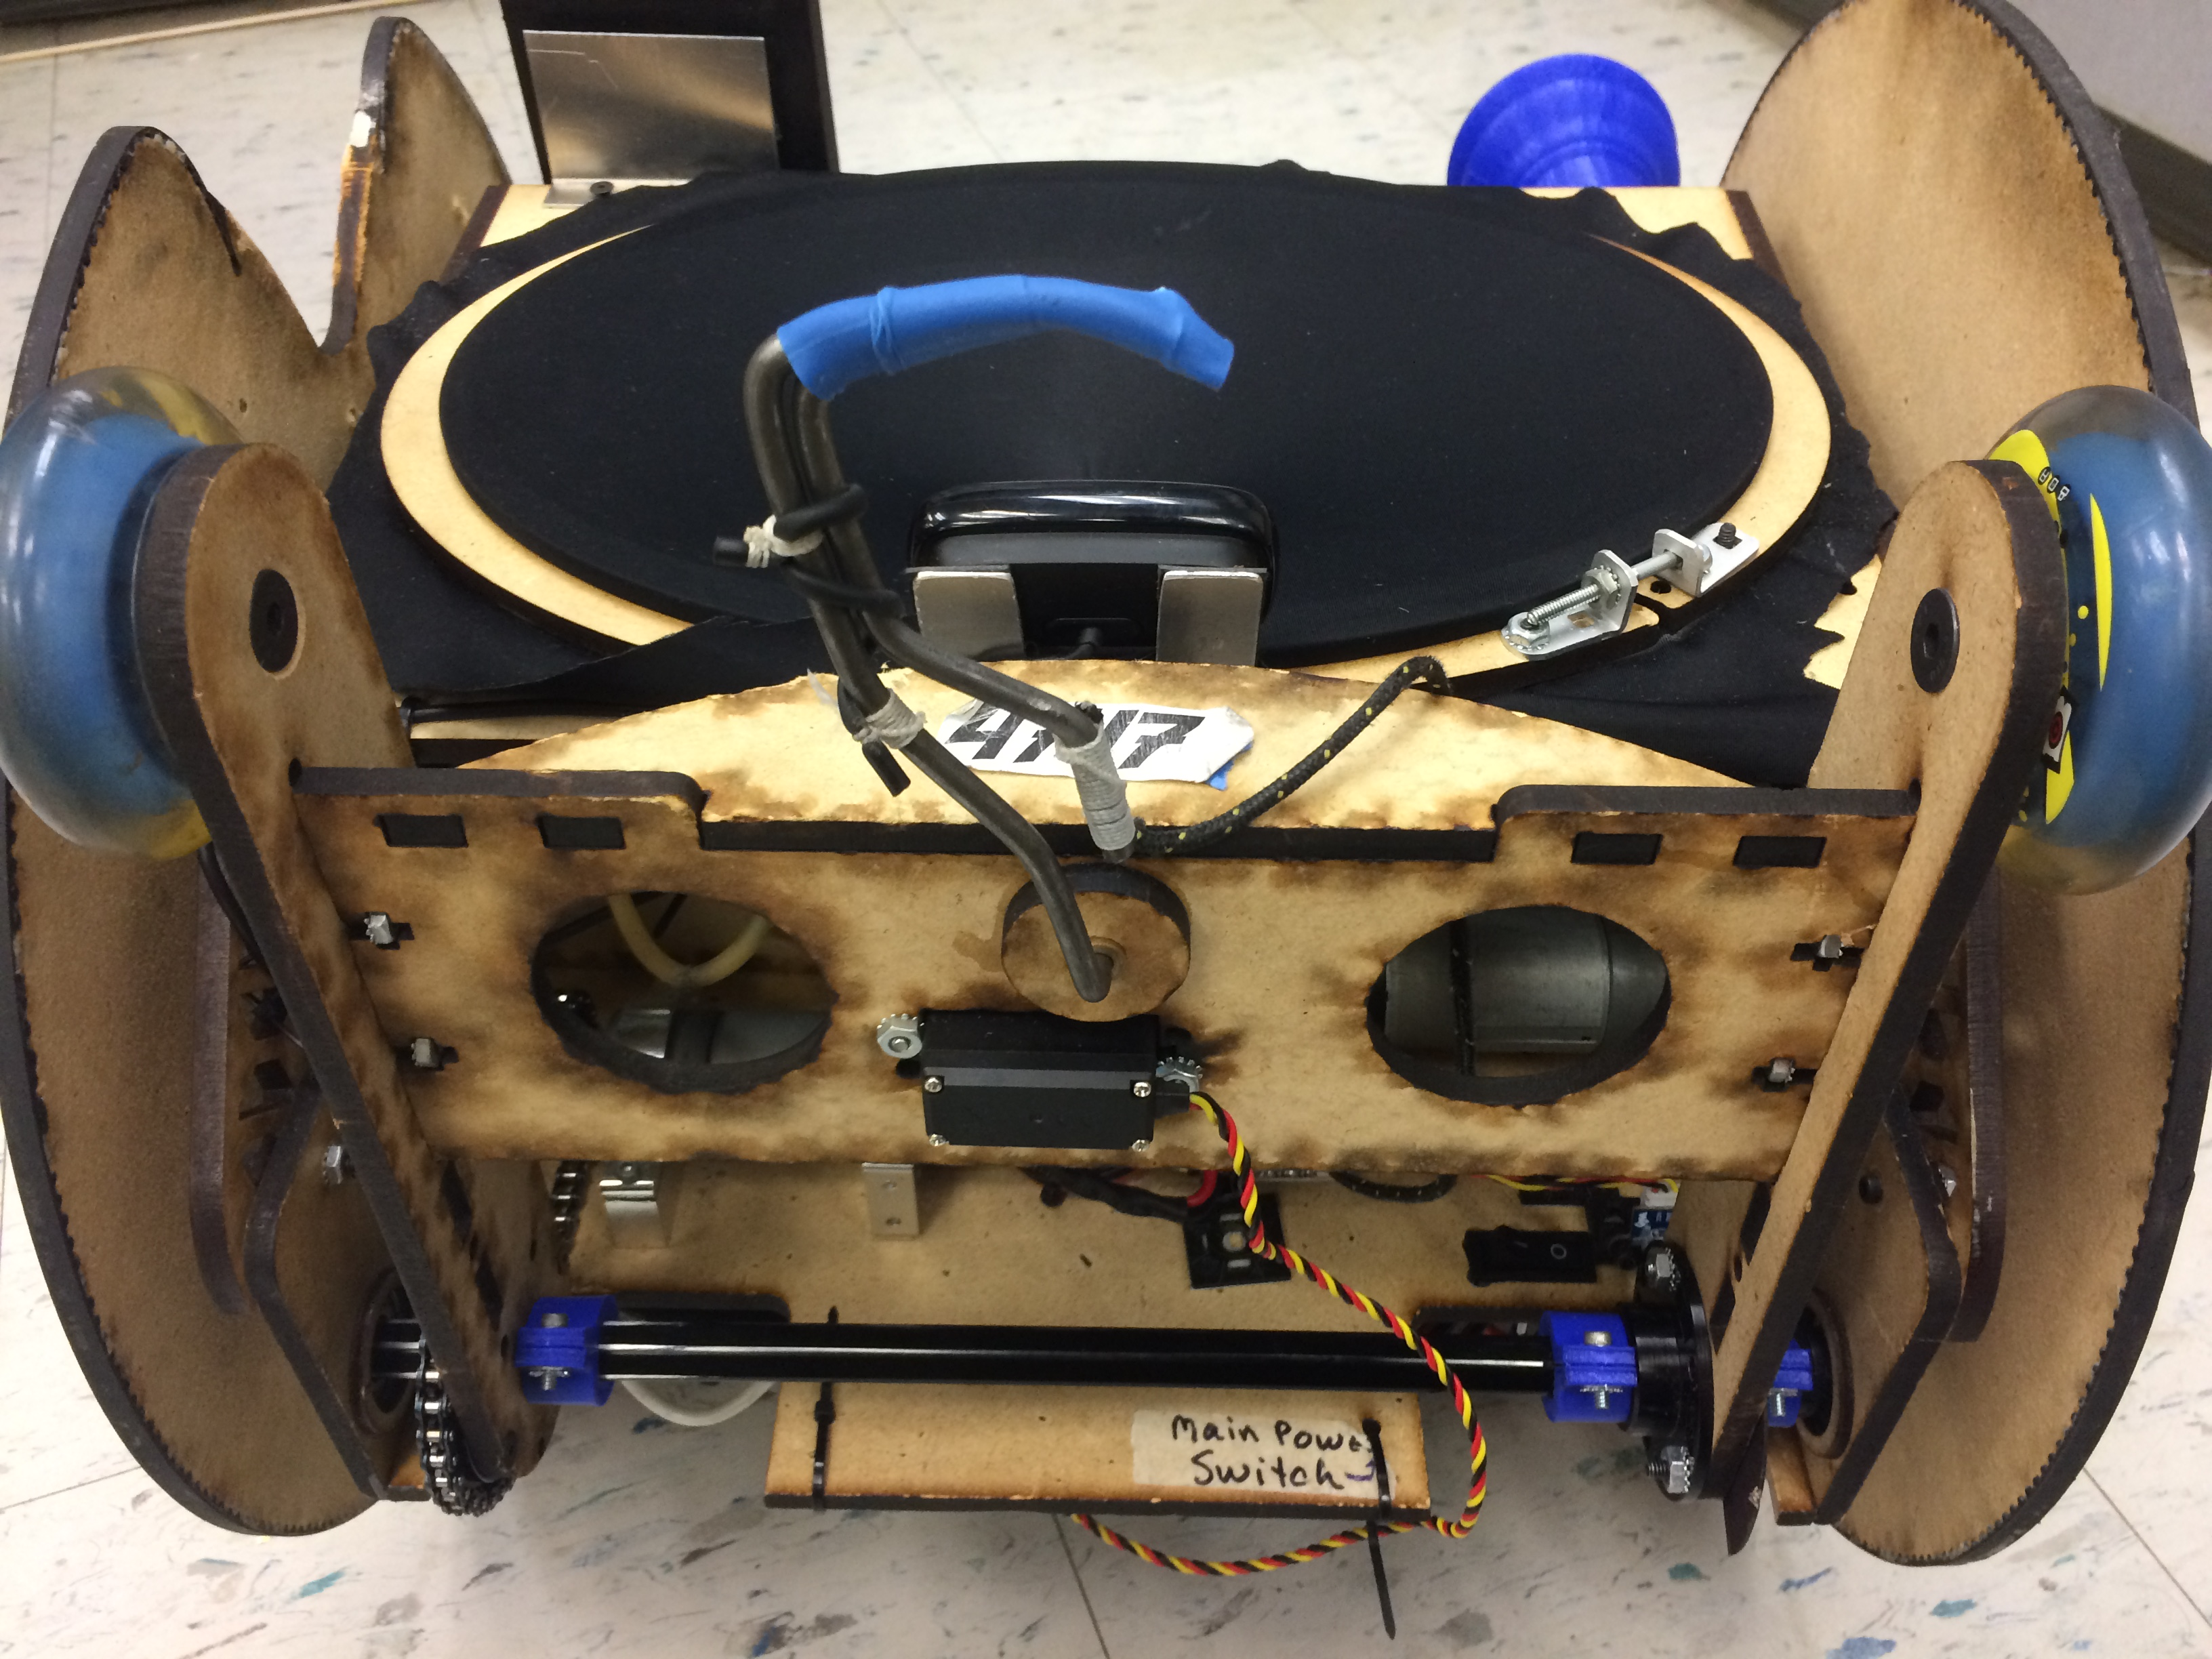
\includegraphics[width= .9\linewidth]{Design_Overview/Hang_Front.JPG}
% 	\caption{Final Hang Mechanism, Mark V}
% 	\label{fig:hang_final_IMG}
% \end{minipage}%
% 	\hfill
% \begin{minipage}{.32\textwidth}
%   \centering
%   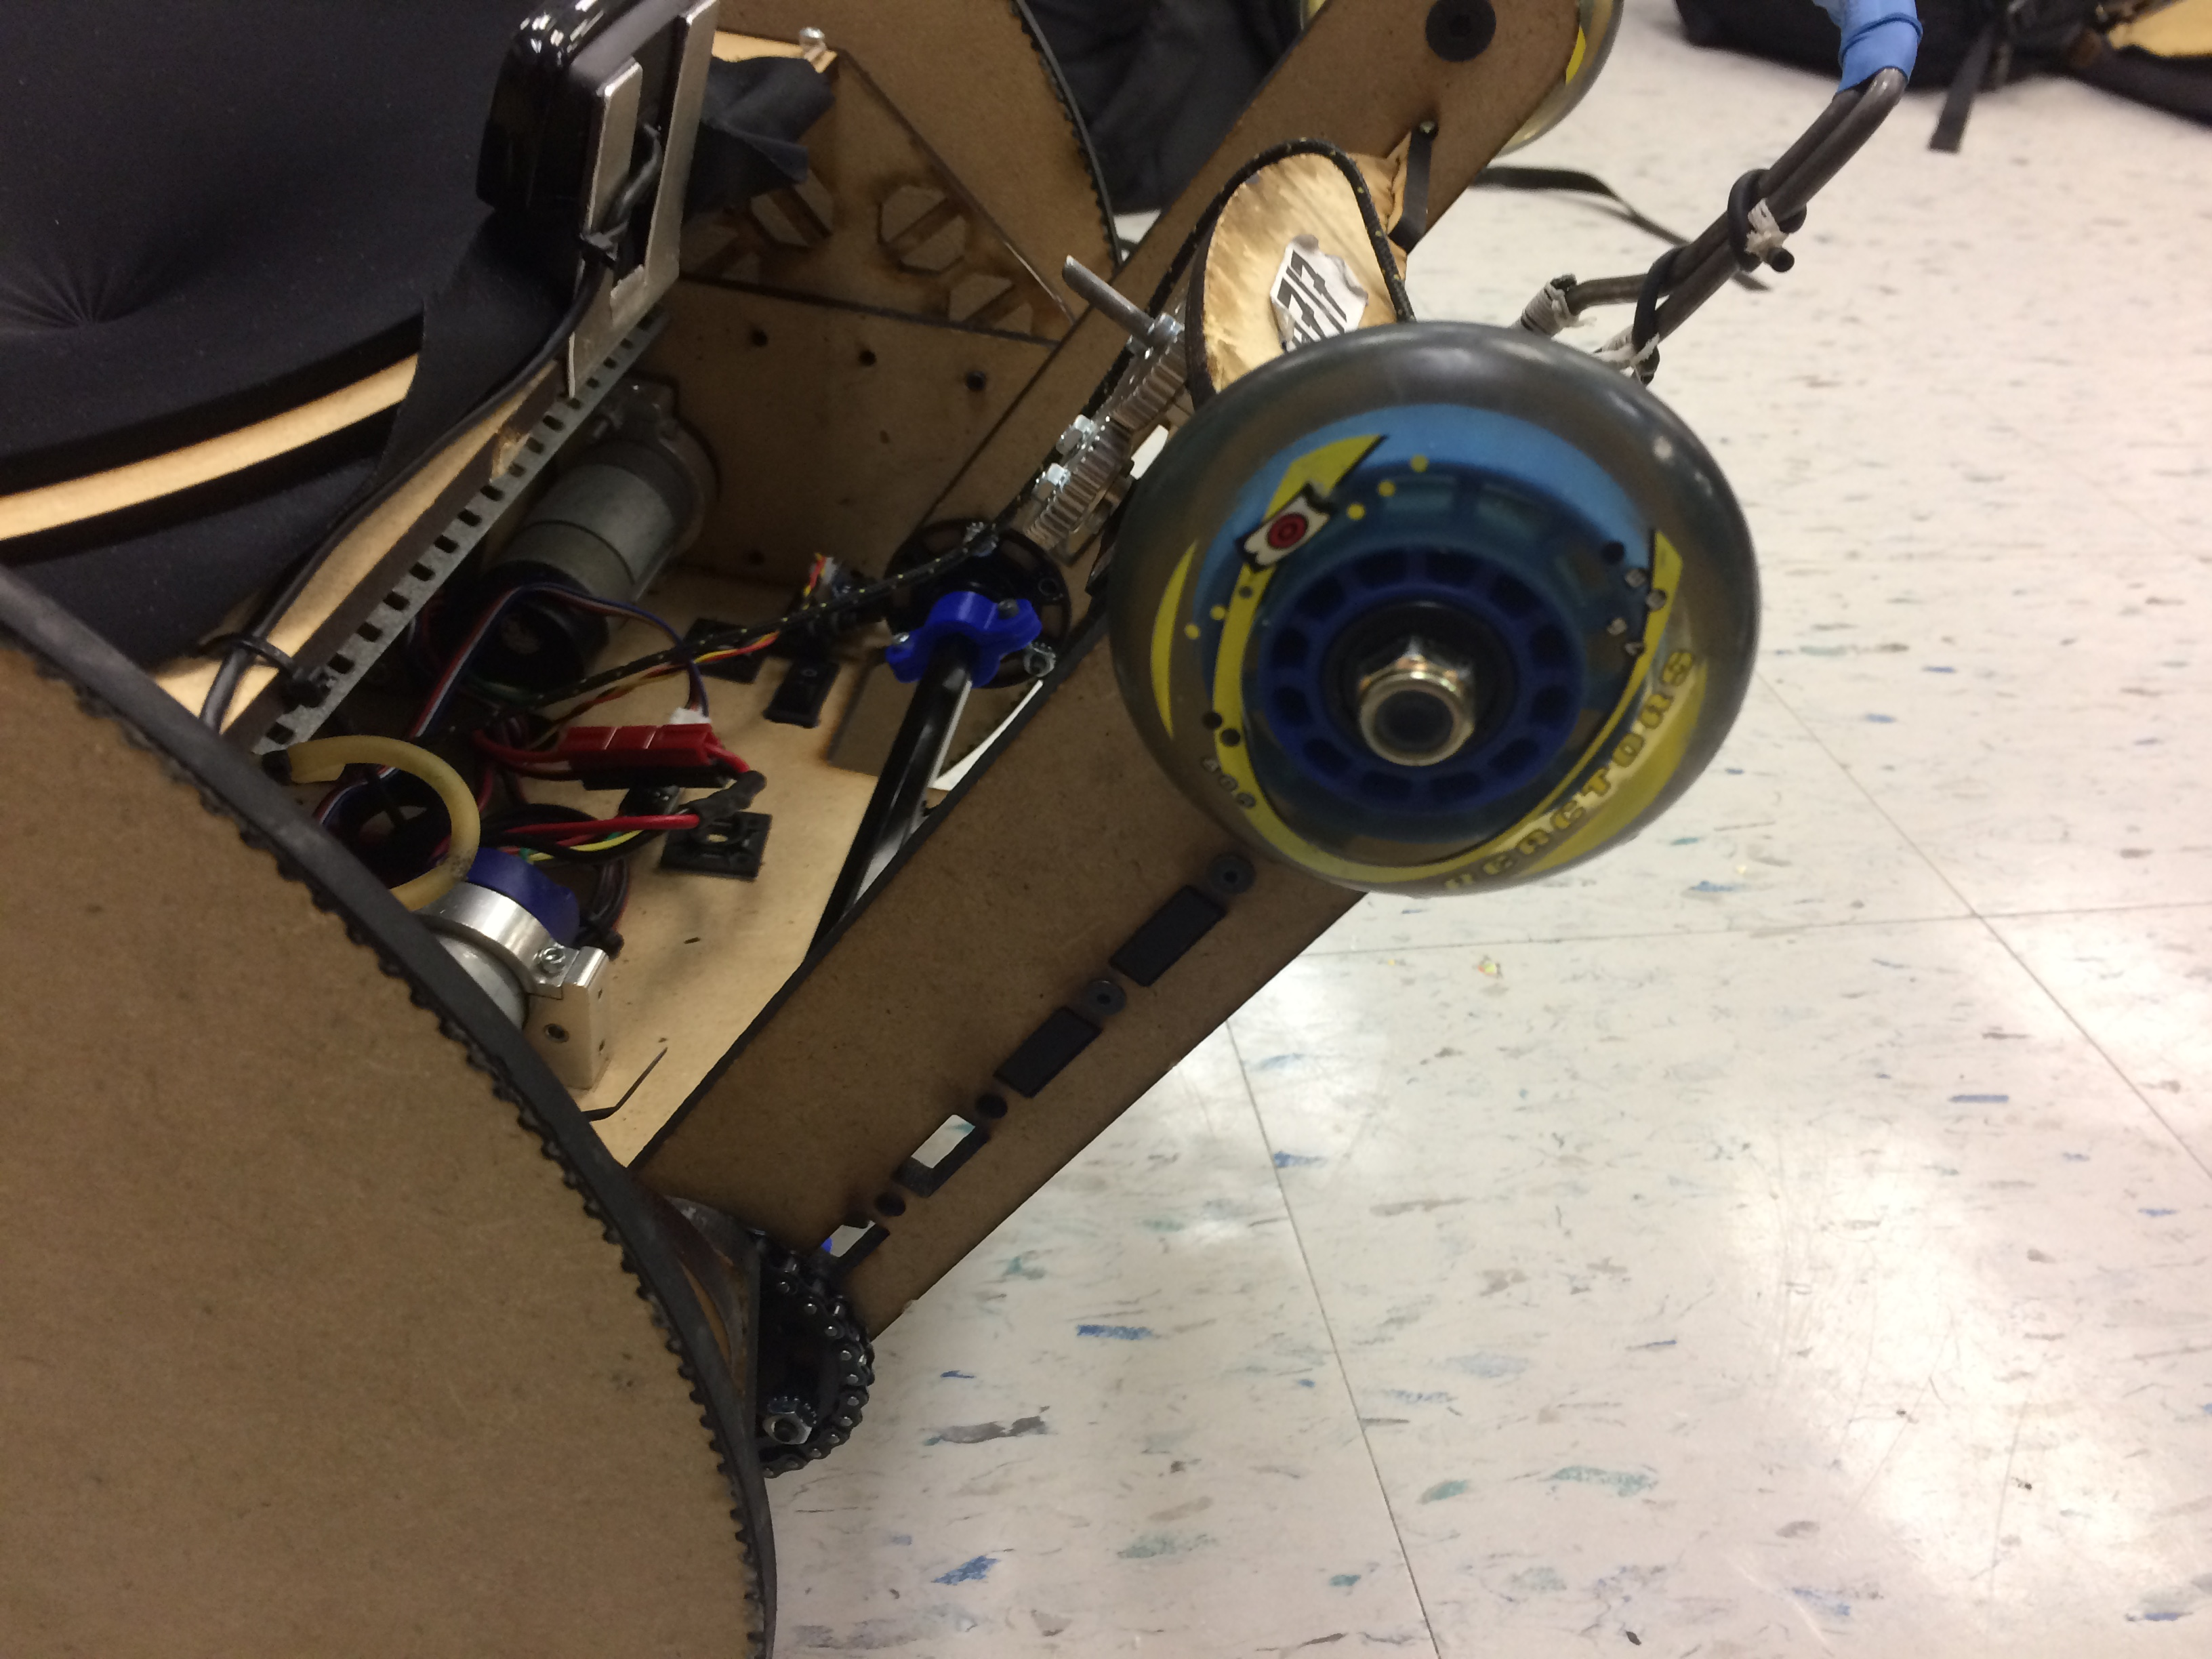
\includegraphics[width= .9\linewidth]{Design_Overview/Hang_Right.JPG}
% \end{minipage}
% \end{figure}

\subsection*{Sensors and Control}
As mentioned before, our team strives to use as many sensors as possible to establish consistency with a high level control. For our Duck Spinner mechanism, you may not think that we would use a sensor here, however we measure the current of our motor to detect when we have arrived at the carousel. Initially, we had a problem with this as we would sometimes get a value above the preset threshold and it would throw our whole program off. To combat this, we used a complex algorithm called a “rolling average,” which constantly cycles new values within an array. With this data, we compute the mean of the last 10 current values to make sure no outliers affect our consistency. In addition, we have developed a machine vision algorithm that is used to drive towards the carousel with speed and consistency. This is primarily used during tele-op to assist our driver. Additionally, we use mathematics to accelerate the duck spinner, which allows us to get all 10 ducks in 21 seconds. Images showing the graph of the current are shown below.

% Image: Design_Spinner_CurrentGraph



\subsection*{Mechanism Accomplishments}
\begin{itemize}
    \item consistently scores 10 ducks 
    \item low center of mass 
    \item optimal velocity for duck control
\end{itemize} 

